  \documentclass[12pt]{article}

  \usepackage[fleqn]{amsmath}
  \usepackage{color}
  \usepackage{listings}
  \usepackage[margin=1in]{geometry}
  \usepackage{indentfirst}
  \usepackage{graphicx}
  \usepackage{float}

  \begin{document}

  \begin{center}
  \vspace*{\fill}
  {\Large\bf University of Waterloo}\\
  \vspace{3mm}
  {\large\bf SE464 Fall 2017}\\
  \vspace{3mm}
  {\Large\bf Prototype Status Update}\\
  \vspace{5mm}
  {\Large Project Name: WatNotes}\\
  \vspace{5mm}
  Michael Socha, Mitchell Kember, Do Gyun Kim, Myungheon Chun\\
  \vspace{3mm}
  msocha@edu.uwaterloo.ca, mkember@edu.uwaterloo.ca, dg3kim@edu.uwaterloo.ca, m5chun@edu.uwaterloo.ca\\
  \vspace*{\fill}
  \end{center}

  \newpage

\section{Status update}
  WatNotes is intended to be a University-wide platform for students to upload, share, and collaboratively edit notes. \\

  Although it was priorly decided that WatNotes would support an Android client and a website, specific implementation technologies had not yet been finalized. For the Android client, the team decided to use Java as the main implementation language, since alternatives such as React Native and Kotlin still seem to be somewhat immature technologies. React was chosen as the primary framework for the website, since it is good at breaking down large websites into modular components. For the backend, Python with PostgreSQL were chosen at the main development technologies. Python is well-known among members of the group, and also has a reputation for encouraging clear, readable code. PostgreSQL is one of the most popular relational database systems, making it a good fit for WatNotes' data, which the team determined in preliminary schema design to be mostly relational. \\

  To build the prototype of the project, the development team split into three small sub-teams, namely backend, mobile, and web. The backend team implemented two main endpoints - one for uploading various types of notes (e.g. .pdf, .txt, images), and another for retrieving these notes to view in a feed. The mobile team setup the core architecture of the Android app and implemented note uploading to the backend. The web team setup the website's core architecture and implemented a feed in which to view notes. Some technical problems were encountered by the development team, such as determining how to effectively store note files in PostgreSQL. Such technical problems can typically be overcome through research to gain a better understanding of the technologies being used. \\

Although the key functionality of note uploading, sharing, and viewing has been implemented, other key features of WatNotes are still missing. For example, collaborative note editing has not been implemented, and the search system will need major improvements to allow for searches by fields such as course and uploader. Development over the next month will focus on these key features, as well as some extension features such as allowing users to rate other notes, and applying NLP to automatically tag notes based on their content.

\section{Demo description}
  The demo will be composed of two stages:
  \begin{enumerate}
    \item Some sample notes will be uploaded using the Android client. Both taking a picture of notes and then uploading the resulting file will be demonstrated, as well as uploading existing files. Uploads of several different file formats (e.g. .txt file, .pdf file, image files) will be demonstrated.

    \item The uploaded notes will be viewed on the feed of the web client.
  \end{enumerate}

  Collaborative note editing functionality is not yet implemented - any note editing during the demo will be simulated.

  \newpage

\section{Architectural overview}
The architecture of WatNotes includes the following components:
\begin{itemize}
\setlength\itemsep{0pt}
  \item Web client (JavaScript, React)
  \item Web server (JavaScript, Node.js)
  \item Android application (Java, Android SDK)
  \item Back end server (Python, Flask)
  \item Data storage (SQLAlchemy, PostgreSQL)
  \item Search system (Elasticsearch)
\end{itemize}
These components, along with the connectors that join them and the topology they form, are shown in the architectural diagram:
\begin{figure}[H]
  \centering
  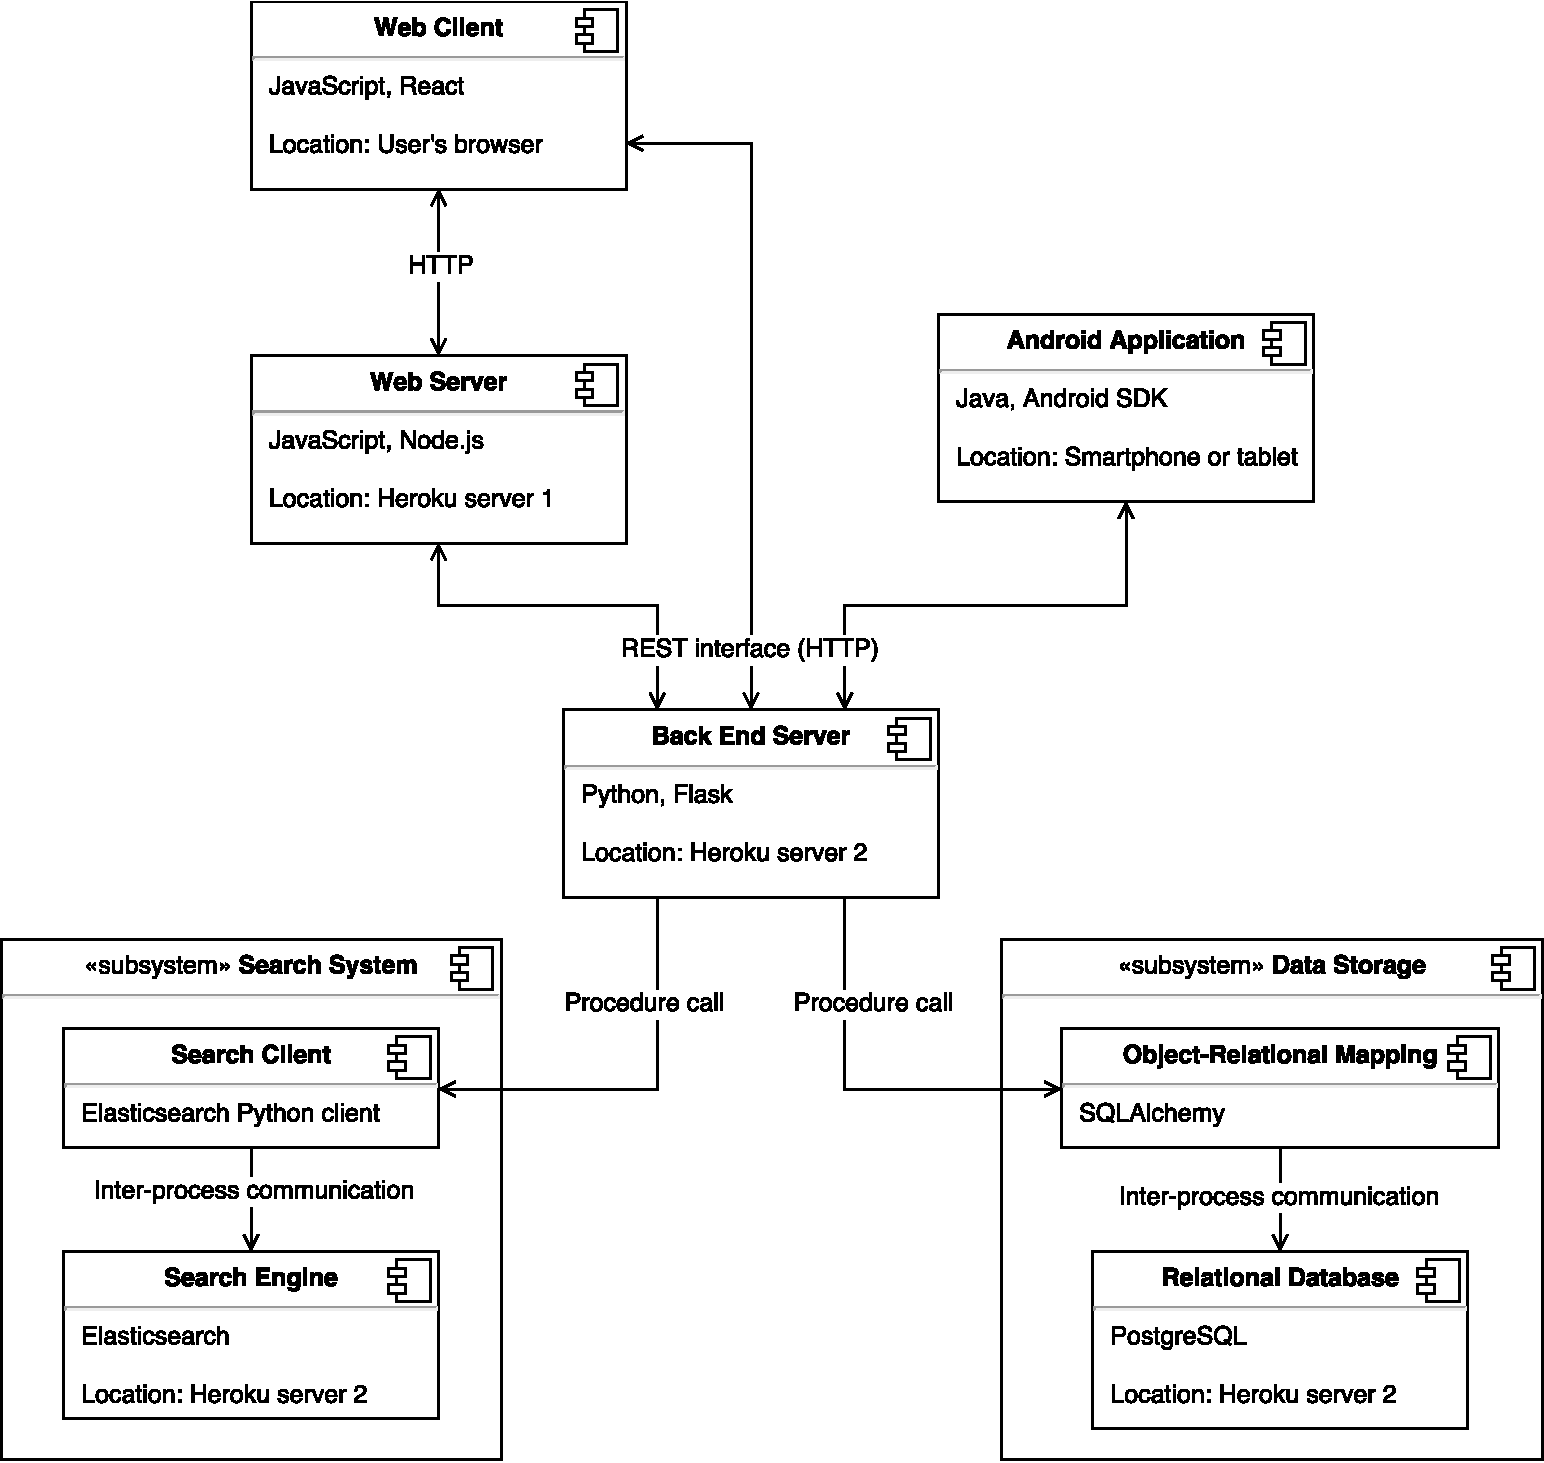
\includegraphics[width=0.9\linewidth]{diagram.pdf}
  \caption{Architectural diagram for WatNotes}
\end{figure}

\end{document}
